\documentclass[border=1pt]{standalone}
\usepackage{tikz}
\usetikzlibrary{calc}

\begin{document}
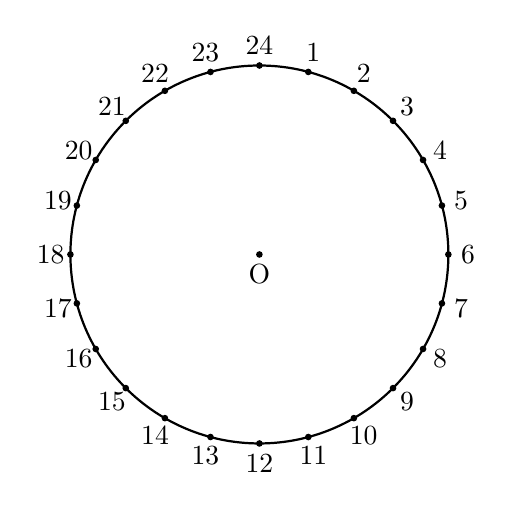
\begin{tikzpicture}
    % 円を描画
    \pgfmathsetmacro{\r}{2.4}
    \draw [thick] (0,0) circle [radius=\r];
    
    % 1-24の数字を円周上に配置（時計的に24が上）
    \pgfmathsetmacro{\n}{24}  
    \foreach \i in {1,2,...,\n} {
        \pgfmathsetmacro{\angle}{90 - \i * 360/\n} 
        \node at (\angle:{\r+0.25}) {\i};
        \fill (\angle:\r) circle (1.2pt); 
    }
    
    % 中心に「O」とマーク
    \fill (0,0) circle (1.2pt) node[below] {O};
    %
\end{tikzpicture}
\end{document}
